\documentclass[a4paper,10pt]{scrbook}
\usepackage{etex}
\usepackage[T1]{fontenc}
\usepackage{geometry}
\usepackage[utf8x]{inputenc}
\usepackage[ngerman]{babel}
\usepackage{graphics}
\usepackage{graphicx}
\usepackage{amssymb}
\usepackage{amsmath}
\usepackage{listings}
\usepackage{booktabs}
\usepackage{pdfpages}
\usepackage{pgfplots}
\usepackage{float}
\usepackage{latexsym}
\usepackage{longtable}
\usepackage{latexsym}
\usepackage{paralist}
\usepackage{pstricks}
\usepackage{stmaryrd}
\usepackage{MnSymbol}
\usepackage{array}
\usepackage{linearb}
\usepackage{titlesec}
\usepackage{listings}
\usepackage{xcolor}
\usepackage{xspace} 
\usepackage{hyperref} 
\usepackage{enumitem}

%Für Arrow listen
\newlist{arrowlist}{itemize}{1}
\setlist[arrowlist]{label=$\rightarrow$}

%Mehr Raum zwischen subsections
\titlespacing{\section}{0pt}{*4}{*2.5}
\titlespacing{\subsection}{0pt}{*3.5}{*1.5}

% kleine Anpassungen, damit die Seitenbreite überall außer Titel gleich ist.
\setcounter{secnumdepth}{2}
\setlength{\textwidth}{160mm}
\setlength{\textheight}{220mm}
\setlength{\headheight}{3mm}
\evensidemargin1mm
\oddsidemargin1mm
%verhindert den wiederlichen Einzug bei einer neuen Zeile
\setlength{\parindent}{0em} 

%Subsections werden hiermit nicht in das Inhaltsverzeichnis übernommen
\setcounter{tocdepth}{1}


%Dokumentenanfang mit diversen input von mehreren Einzeldokumenten.
\begin{document}
	\begin{titlepage}
\center
\Large Datenbanken 1 Lernskript \\[2em]
Dozent:\\Pro. Dr. Stefan Kramer \\[2em]
\LaTeX{} von:\\Sven Bamberger\\[2em]
Zuletzt Aktualisiert:\\\today\\

\includegraphics[scale=.2]{front/pics/Logo.jpg}\\\quad\\
\end{titlepage}
 
	
	\frontmatter 
		Dieses Skript wurde erstellt, um sich besser auf die Klausur vorzubereiten.\\
\qquad\\
\qquad\\
\textcolor{red}{\Large{Dieses Dokument garantiert weder Richtigkeit noch Vollständigkeit, da es aus Mitschriften und Vorlesungsfolien gefertigt wurde und dabei immer Fehler entstehen können. Falls ein Fehler enthalten ist, bitte melden oder selbst korrigieren und neu hoch laden.}}


		 
\tableofcontents 
 
	 
	\mainmatter 
		\chapter{Allgemeines}
\section{Klausurtermin}
Die Klausur findet am 14.08.2014 in Raum N1 und/oder N3 statt.

\section{Material für die Klausur}
Bis zum aktuellen Zeitpunkt sind keine Hilfsmittel zugelassen
%
\section{Empfohlene Lektüre:}
Für die Vorlesung wird das folgende Buch dringend empfohlen, da sich die Vorlesung an diesem orientieren wird. \\
Datenbanksysteme: Eine Einführung\\
 Autoren: Alfons Kemper, André Eickler\\
 Auflage: 9.\\
 Oldenbourg Wissenschaftsverlag\\
(25. September 2013)\\
ISBN-10: 3486721399\\
ISBN-13: 978-3486721393\\

Die Auflage Nummer 8 wird für die Übungen verwendet. Auch Auflage 7 kann noch ausreichend sein. Jedoch ist dieses Buch äußerst lange aktuell und es lohnt sich dieses anzuschaffen. In dieser Vorlesung wird Kapitel 1 - 9 behandelt, wobei ein paar Themenbereiche wie z.B. JDBC ausgelassen werden. 

\subsection{Weiterführende Lektüre/Links:}
\begin{enumerate}
\item A. Silberschatz, H. F. Korth und S. Sudarshan Database System Concepts, 4. Auflage, McGraw-Hill Book Co., 2002.
\item R. Elmasri, S.B. Navathe: Fundamentals of Database Systems, Benjamin Cummings, Redwood City, Ca, USA, 2. Auflage, 1994
\item R. Ramakrishnan, J. Gehrke: Database Management Systems, 3. Auflage, 2003.
\item G. Vossen : Datenmodelle, Datenbanksprachen und Datenbank-Management-Systeme. Oldenbourg, 2001.
\item \textbf{D. Maier: The Theory of Relational Databases. Computer Science Press. 1983.}
\item S. M. Lang, P.C. Lockemann: Datenbankeinsatz. Springer Verlage, 1995.
\item C. Batini, S. Ceri, S.B. Navathe: Conceptual Database Design, Benjamin Cummings, Redwood City, Ca, USA, 1992.
\item \textbf{C. J. Date: An Introduction to Database Systems. McGraw-Hill, 8. Aufl., 2003.}
\item J.D. Ullmann, J. Widom: A First Course in Database Systems, McGraw Hill, 2. Auflage, 2001. 8
\item A. Kemper, G. Moerkotte: Object-Oriented Database Management: Applications in Engineering and Computer
Science, Prentice Hall, 1994 
\item E. Rahm: Mehrrechner-Datenbanksyseme. Addison-Wesley, 1994.
\item P. Dadam: Verteilte Datenbanken und Client/Server Systeme. Springer Verlag, 1996
\item G. Weikum, G. Vossen: Transactional Information Systems: Theory, Algorithms, and the Practice of Concurrency Control. Morgan Kaufmann, 2001.
\item T. Härder, E. Rahm: Datenbanksysteme – Konzepte und Techniken der Implementierung, 2001.

\end{enumerate}
\section{Verwendete Software:}
Es wird vorzugsweise auf \href{http://www.postgresql.org/}{PostgreSQL} und \href{http://www.mysql.de/}{MySQL} als OpenSource Varianten zurück gegriffen. Um die Blätter auch ordentlich bearbeiten zu können wird die Installation dieser Systeme empfohlen. 
		\chapter{Einleitung und Übersicht}
\textit{Datenbankverwaltungssysteme} (DBMS) gewinnen dank der digitalen Vernetzung und Kommunikation immer mehr an Bedeutung und sind heutzutage nicht mehr aus unserem Alltag wegzudenken. Zwar bemerken viele den Einsatz eines DBMS nicht jedoch sind diese Systeme überall

\section{Empfohlene Lektüre:}
Für die Vorlesung wird das folgende Buch dringend empfohlen, da sich die Vorlesung an diesem orientieren wird. \\ vertreten z.B. in Versicherungen, Banken, Universitäten (welche das Hauptbeispiel für diese Vorlesung bildet) noch bei vermeintlich nicht aufwendigen Blogs wie einem einfachem Blog.\\
Ein Datenbankverwaltungssystem besteht aus einer Menge von \textit{Daten} und dem \textit{Datenbankverwaltungssystem} 
\begin{itemize}
	\item Die \textit{Daten} werden auch als Datenbasis bezeichnet welche in einer gewissen Beziehung zueinander stehen. 
	\item Die Programme zum Zugriff, Modifikation und Kontrolle genutzt werden, werden als \textit{Datenbankverwaltungssystem} bezeichnet
\end{itemize}
Diese Trennung wird häufig unterlassen, um eine Verwirrung zu vermeiden. Stattdessen werden Datenbankverwaltungssysteme (auch Datenbanksysteme) als Kombination der vorher genannten Unterschiede bezeichnet. 

\section{Motivation für ein DBMS}
Es gibt einige Probleme wenn Firmen oder Organisationen auf ein DBMS verzichten müssten und auf Papier (Karteikarten, Akten, \dots) oder separate Dateien zurück greifen müssten. 
\begin{description}
  \item[Redundanz und Inkonsistenz:] \hfill\\
   Wenn Daten isoliert gehalten werden, müssen diese mehrfach vorhanden sein (Zweigstelle einer Firma) und wenn Informationen in einer dieser Dateien geändert werden, geschieht dies lediglich in dieser einen Dateien, Hierdurch entstehen, aufgrund der vorhandenen Redundanz, Inkonsistenzen in den Informationen. 
  \item[Beschränkte Zugriffsmöglichkeiten:] \hfill \\
  	Es ist nahezu unmöglich separierte Dateien miteinander zu verknüpfen und logische Abhängigkeiten zu generieren. Mit einem DBMS können Informationen einer Firma/Organisation einheitlich modelliert werden (\text{Datenmodell}) . Dadurch lassen sich die Daten auf viele Arten verknüpfen. 
  \item[Probleme beim Mehrbenutzerbetrieb:] \hfill \\
  	Dateisysteme bieten nur wenige Kontrollmechanismen für den Mehrbenutzerbetrieb. Das bedeutet, falls mehrere Benutzer an einer Datei arbeiten, wird bei jedem Speicher Vorgang alle vorherigen Änderungen überschrieben. Dies nennt man ein \glqq{}lost update\grqq{}. DBMS bieten eine Mehrbenutzerkontrolle, welche solche Anomalien erkennt und verhindert. 
  \item[Verlust von Daten:] \hfill \\ 
  	Bei isolierten Daten wird die Wiederherstellung eines konsistenten Zustandes äußerst schwierig. Datenbankverwaltungssysteme haben Möglichkeiten diese Daten wieder herzustellen.
  \item[Integritätsverletzung:]\hfill \\ 
  	Diese \textit{Abhängigkeitsverletzungen} können auftreten, wenn Daten und Informationen isoliert bearbeitet und betrachtet werden. Die Überprüfung auf Integritätsverletzungen sollte vom System geprüft und bei Bedarf abgelehnt werden. DBMS führen Transaktionen nur aus, wenn sie die Datenbasis in eine konsistenten Zustand überführen. 
  \item[Sicherheitsprobleme:] \hfill \\
  	Nicht jeder sollte Zugriff auf alle gespeicherten Daten haben, sondern lediglich auf bestimmte Bereiche und Daten, die unbedingt notwendig sind. Auch sollten nur bestimmte Leute das \textit{Privileg} haben Daten zu verändern oder gar zu löschen. DBMS Systeme haben ausgefeilte Rechteverwaltungen für Benutzer und Benutzergruppen.. 
  \item[hohe Entwicklungskosten für Anwendungsprogramme:] \hfill \\
  	Anwendungsentwickler müssen sich meist mit einem Teil der vorher genannten Probleme auseinandersetzen um Informationen zu speichern und zu verwalten. Ein DBMS bietet eine einfache und erprobte Möglichkeit diese Probleme direkt zu erledigen.
\end{description}

\section{Die Abstraktionsebenen eines Datenbanksystems}
\begin{figure}[h!]
\centering
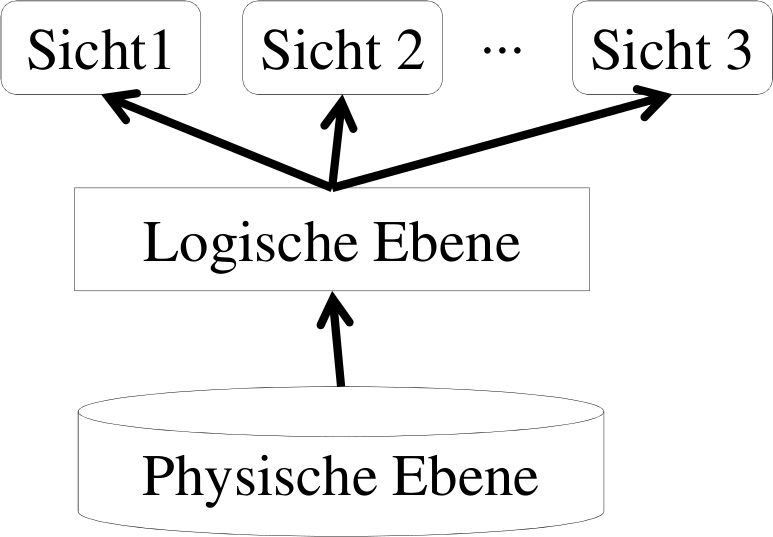
\includegraphics[width=0.45\linewidth]{./mainmatter/pics/sichten}
\caption[Abstraktionsebenen]{Drei Abstraktionsebenen eines Datenbanksystems}
\label{fig:sichten}
\end{figure}
Bei einem DBMS unterscheidet man drei Abstraktionsebenen(siehe Abbildung \ref{fig:sichten}).
\begin{description}
\item[Die physische Ebene:] Auf dieser Ebene wird festgelegt, wie die Daten gespeichert sind. Im Allgemeinen sind die Daten auf einem Speichermedium (meistens als Plattenspeicher realisiert) abgelegt. 
\item[Die logische Ebene:] Auf der logischen Ebene wird in einem sogenannten \textit{Datenbankschema} festgelegt, welche Daten abgespeichert sind. 
\item[Die Sichten:] Während das Datenbankschema der logischen Ebene ein integriertes Modell der gesamten Informationsmenge des jeweiligen Anwendungsbereichs (z.B. des gesamten Unternehmens) darstellt, werden in den Sichten Teilmenge der Informationen bereitgestellt. Diese Sichten sind auf Benutzer bzw. Benutzergruppen zugeschnitten, die lediglich diese Sichten benötigen. Denn nicht jeder Benutzer benötigt alle Daten die existieren.
\end{description}

\section{Datenunabhängigkeit}
Durch die drei Ebenen wird eine Datenunabhängigkeit erreicht, welche zu wohl definierten Schnittstellen führt, ermöglicht es die Realisierung der Datenbank zu variieren ohne die Benutzer der Schnittstellen in Mitleidenschaft zu ziehen. Aus den drei Schichten ergeben sich zwei Stufen der Datenunabhängigkeit im DBMS
\begin{description}
\item[Physische Datenunabhängigkeit:] Die Modifikation der physischen Speicherstruktur belässt die logische Ebene (also das Datenbankschema) invariant. Z.B. erlauben fast alle Datenbanksysteme das nachträgliche Anlegen eines Indexes, um die Datenbankobjekte schneller finden zu können. Dies darf keinen Einfluss au bereits existierende Anwendungen in der logischen Ebene haben. Es sollte lediglich die Effizienz positiv beeinflussen.
\item[Logische Datenunabhängigkeit:] Die Anwendungen nehmen stets Bezug auf die logische Struktur der Datenbasis. Bei Änderungen der logischen Ebene (des Datenbankschemas) können diese in den Sichten vor dem Anwender verborgen werden. Dadurch wird zu einem gewissen Grad eine logische Datenbankunabhängigkeit erzielt. 
\end{description}
Die heutigen Datenbanksysteme erfüllen mindestens die physische Datenbankunabhängigkeit. Die logische Datenunabhängigkeit kann schon rein konzeptuell nur für einfachste Modifikationen des Datenbankschemas gewährleistet werden. 
\section{Datenmodellierung}
	\backmatter
		\listoffigures 
\end {document}
